% ============================================================
% sections/results.tex  結果（初稿 2026-10-26）
% 数字はプロジェクトの md にあるものだけ。各段落の末尾のコメントに出どころを書く（第2弾の照合用）。
% 組の名前：組1=s0，組2=s1，組3=s2（本番），組4=s3（予備），組5=s4，組6=s5（追加）。
% 「範囲」は最終5点の平均を組ごとにとった値の，組の間の最小〜最大（特に断らない限り）。
% ============================================================
\section{結果}\label{sec:results}

\subsection{実験1：自分側の見込み}\label{sec:res-self}

\begin{figure}[t]
  \centering
  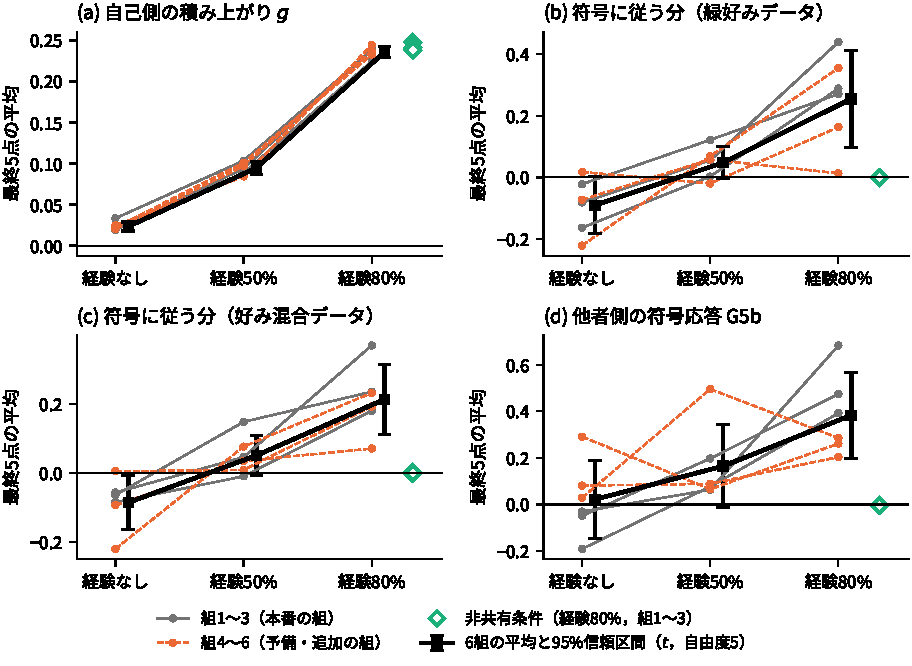
\includegraphics[width=\linewidth]{figs/central}
  % 図3（中心の図）：4パネル。横軸は経験なし・経験50%・経験80%，縦軸は最終5点の平均。
  % (a) 自分側の積み上がり g（実験1），(b) 符号に従う分（緑好みデータ），(c) 符号に従う分（好み混合データ），
  % (d) 他者側の符号応答 G5b（(b)〜(d) は実験2）。
  % 各組を細い線（組1〜3 は灰色の実線，組4〜6 は橙の破線），6組の平均と t の 95% CI（自由度5）を太い黒，
  % 非共有条件（組1〜3）を経験80% の横に白い菱形。
  % 元：data/result/v13/compare_all/figs/central_v13.png（v13 まとめ §11）
  \caption{経験の量と共有の有無による，自分側と他者側の見込みの強さ．細い線は各組，太い線は6組の平均と95\%信頼区間，白い菱形は非共有条件（組1〜3）を表す．組1〜3 は灰の実線，組4 は橙の破線，組5・6 は橙の点線と白抜きの四角で示す．(a) 自分側の積み上がり $g$（事前登録）．(b)(c) 他者側の符号に従う分（緑好みデータ，好み混合データ．組1〜4 では事後に定義し，組5・6 は事前登録）．(d) 他者側の符号応答 G5b（事前登録）．}
  \label{fig:central}
\end{figure}

\begin{table}[t]
  \centering
  \small
  \caption{組ごとの値と組をまたいだ差}
  \label{tab:group_values}
  % paper/tables/group_values.tex -- generated by analyze/paper/tables_paper.py; sources in paper/tables/README.md
\begin{tabular}{@{}lll@{}}
\toprule
 & 自己側の積み上がり $g$ & 符号に従う分（緑好み） \\
\midrule
\multicolumn{3}{@{}l}{組ごとの値（最終5点の平均．経験なし / 経験50\% / 経験80\%）} \\
組1 & $+0.019$ / $+0.094$ / $+0.240$ & $-0.022$ / $+0.122$ / $+0.270$ \\
組2 & $+0.033$ / $+0.103$ / $+0.238$ & $-0.081$ / $+0.055$ / $+0.438$ \\
組3 & $+0.021$ / $+0.089$ / $+0.225$ & $-0.163$ / $+0.003$ / $+0.288$ \\
組4 & $+0.024$ / $+0.084$ / $+0.244$ & $-0.072$ / $+0.058$ / $+0.013$ \\
組5 & $+0.022$ / $+0.101$ / $+0.233$ & $+0.018$ / $-0.020$ / $+0.163$ \\
組6 & $+0.020$ / $+0.097$ / $+0.237$ & $-0.221$ / $+0.069$ / $+0.354$ \\
非共有（組1 / 組2 / 組3） & $+0.248$ / $+0.241$ / $+0.238$ & $-0.001$ / $-0.000$ / $-0.001$ \\
\multicolumn{3}{@{}l}{組をまたいだ差（6組の平均 [95\%信頼区間]，$t$ 分布，自由度5）} \\
経験50\% $-$ 経験なし & $+0.071$ [$+0.064$, $+0.079$] & $+0.138$ [$+0.028$, $+0.248$] \\
経験80\% $-$ 経験50\% & $+0.141$ [$+0.131$, $+0.152$] & $+0.207$ [$+0.050$, $+0.363$] \\
経験80\% $-$ 経験なし & $+0.213$ [$+0.205$, $+0.221$] & $+0.345$ [$+0.132$, $+0.557$] \\
\midrule[\heavyrulewidth]
 & 符号に従う分（好み混合） & 他者側の符号応答 G5b \\
\midrule
\multicolumn{3}{@{}l}{組ごとの値（最終5点の平均．経験なし / 経験50\% / 経験80\%）} \\
組1 & $-0.065$ / $+0.148$ / $+0.235$ & $-0.049$ / $+0.197$ / $+0.474$ \\
組2 & $-0.057$ / $+0.046$ / $+0.370$ & $-0.030$ / $+0.063$ / $+0.682$ \\
組3 & $-0.086$ / $-0.010$ / $+0.180$ & $-0.191$ / $+0.077$ / $+0.392$ \\
組4 & $-0.094$ / $+0.034$ / $+0.071$ & $+0.291$ / $+0.066$ / $+0.261$ \\
組5 & $+0.005$ / $+0.008$ / $+0.192$ & $+0.081$ / $+0.089$ / $+0.204$ \\
組6 & $-0.221$ / $+0.076$ / $+0.232$ & $+0.029$ / $+0.495$ / $+0.285$ \\
非共有（組1 / 組2 / 組3） & $-0.002$ / $+0.002$ / $-0.000$ & $-0.002$ / $-0.005$ / $-0.005$ \\
\multicolumn{3}{@{}l}{組をまたいだ差（6組の平均 [95\%信頼区間]，$t$ 分布，自由度5）} \\
経験50\% $-$ 経験なし & $+0.137$ [$+0.027$, $+0.246$] & $+0.143$ [$-0.109$, $+0.394$] \\
経験80\% $-$ 経験50\% & $+0.163$ [$+0.059$, $+0.267$] & $+0.218$ [$-0.066$, $+0.503$] \\
経験80\% $-$ 経験なし & $+0.300$ [$+0.174$, $+0.425$] & $+0.361$ [$+0.057$, $+0.665$] \\
\bottomrule
\end{tabular}

  % 表3：G3・符号に従う分（2データ）・G5b の，組1〜6 の経験なし・50%・80% の値（最終5点の平均），
  % 非共有条件（組1〜3）の値，組をまたいだ差（50%−経験なし，80%−50%，80%−経験なし）の平均と 95% CI。
  % 出典：v13 まとめ §3 表3・§6 表6・§11。
\end{table}

前提として確かめた自己位置の追跡は，経験50\%条件では6組すべてで基準（決定係数 0.80）を満たした．
経験80\%条件は6組とも基準に届かなかった．
共通テスト（ランダムに歩くデータ）では 0.70〜0.75（本番の3組では 0.72〜0.75）であったが，自分の学習データと同じ作りのテストでは 0.99 であり，角にとどまる学習データの偏りによる，経験していない場面への一般化の弱さと考えられる．
% 出典：v13 まとめ §3（G1 の不足）・§10 表（G1 80% 0/6，50% 6/6）。
事前登録した手続きでは，この前提は段階IIへ進む条件であり，経験80\%条件の段階IIは，この前提と G5a の関門を満たさなかったため探索として行った（\ref{sec:res-module}節）．
実験1・2・4 の指標は内部状態からの位置の読み出しを使わず，モデル自身の予測から測るので，追跡が基準に届かないことはこれらの指標の計算を妨げない．
ただし，経験80\%条件のモデルは共通テストの場面に十分には一般化していない状態にあり，以下の経験80\%条件の値は，その状態を含んだものとして読む必要がある．
運動が隠れたステップで予測が赤の方へ一歩動いた場合の視界に寄るか（\ref{app:gates}）は，経験50\%条件・経験80\%条件とも6組すべてで成り立った．
% 出典：v13 まとめ §10 (a) G2。

主の指標である自分側の積み上がり $g$ は，経験の量に応じて段階的に大きくなった（図\ref{fig:central}(a)，表\ref{tab:group_values}）．
本番の3組の値は，経験なし条件で $+0.019$〜$+0.033$，経験50\%条件で $+0.089$〜$+0.103$，経験80\%条件で $+0.225$〜$+0.240$ であった．
組ごとの事前登録した判定では，経験50\%条件・経験80\%条件とも経験なし条件との差が6組すべてで成り立ち，同じ組の中で経験80\%条件が経験50\%条件を上回ることも6組すべてで成り立った．
組をまたいだ差（6組）は，経験50\%条件 $-$ 経験なし条件が $+0.071$ [$+0.064$, $+0.079$]，経験80\%条件 $-$ 経験50\%条件が $+0.141$ [$+0.131$, $+0.152$]，経験80\%条件 $-$ 経験なし条件が $+0.213$ [$+0.205$, $+0.221$] で，どの段階でも信頼区間は0を含まなかった．
% 出典：v13 まとめ §6 表6（G3 の範囲，本番3組），§10 (a)(b)，§11 表（G3）。
角から離れた場面だけを取り出しても，同じ向きで同程度の大きさであり，角の近くだけで働く形ではなかった．
% 出典：v13 まとめ §3（角の近くかどうかで分けた記述）。

非共有条件でも，自分側の見込みは経験80\%条件と同じように生まれた．
非共有条件の $g$ は $+0.238$〜$+0.248$（組1〜3）で，同じ組の経験80\%条件との差は $-0.02$〜$+0.03$ にとどまり，次の視界の予測誤差の違いも 10\% 以内であった．
自分側の見込みは，自他で重みを共有するかどうかによらず学習される．
% 出典：v13 まとめ §5（自分側は v13 と同程度），§6 表6（NS の G3）。
以上より H1 は支持された．
ただし経験なし条件の $g$ も小さく正であり（本番の3組で $+0.019$〜$+0.033$），H1 の「経験があるとき」は，経験なし条件よりはっきり強いという意味で支持された．
自己位置の追跡の前提を満たした経験50\%条件と経験なし条件の比較だけでも，見込みが経験によって生まれることは6組すべてで成り立つ．
一方，経験が多いほど強いという部分は，前提を満たさなかった経験80\%条件に依っている．

ただし，ここでの経験の効果は，学習データの位置の分布の変化と分けられていない．
規則の割合を上げると，赤から距離5以内にいるフレームの割合も約0.03，約0.33，約0.85と大きく変わる（\ref{sec:env}節）．
角から離れた場面でも同じ向きの結果が得られたことは，角の近くだけで働く形ではないことを示すが，学習時の分布の違いによる影響を除くものではない．
価値に従って動いた経験そのものの効果と，特定の場所に多くいた経験の効果を分けるには，位置の分布をそろえて価値と行動の結びつきだけを変える対照が要る（\ref{sec:future}節）．
また，経験の量は3水準だけであり，強まり方が比例的か飽和的かは分からない．

\subsection{実験2：他者側への当てはめ}\label{sec:res-other}

\paragraph{他者側の符号応答（事前登録した主の指標）}
process-2 の一つの範囲に快 $+a$ と不快 $-a$ を入れると，経験80\%条件では予測の中の A-2 がその向きにずれた（図\ref{fig:central}(d)）．
本番の3組では，経験80\%条件の G5b は $+0.392$〜$+0.682$（経験なし条件 $-0.191$〜$-0.030$）で，3組とも5点すべてで経験なし条件との差が成り立ち，事前登録した判定に合格した．
経験50\%条件の G5b は $+0.063$〜$+0.197$ で，合格は3組中2組であった．
ずれは段階Iで快・不快が0以外になる範囲 0・1・6・7 に集まり，範囲 2〜5 ではほぼ0であった．
% 出典：v13 まとめ §6 表6（G5b），§3.1（v12 2/3 組：s0 5/5，s1 2/5，s2 3/5），§8 の 3（g5b_bins）。

全6組では，経験80\%条件と経験なし条件の差は6組中5組で成り立ち，組をまたいだ差は $+0.361$ [$+0.057$, $+0.665$] で0を含まなかった．
一方，段階ごとの差は，経験50\%条件 $-$ 経験なし条件が $+0.143$ [$-0.109$, $+0.394$]，経験80\%条件 $-$ 経験50\%条件が $+0.218$ [$-0.066$, $+0.503$] で，どちらも0を含んだ．
したがって G5b で示せるのは，経験80\%条件の他者側の働きが経験なし条件より大きいことまでであり，段階的な強まりは示せていない．
外れた組は二つある．
組4では経験なし条件の G5b が $+0.291$ と大きく，経験80\%条件との差が出なかった．
組6では経験50\%条件（$+0.495$）が経験80\%条件（$+0.285$）を上回った（\ref{app:component}）．
% 出典：v13 まとめ §10（(c) G5b 80%−経験なし 5/6），§11 表（G5b），§3 表3（s3・s5）。

\paragraph{符号に従う分}
A-2 の本当の快・不快を保って入れた場合と，その符号を反転して入れた場合の差（符号に従う分）でも，同じ向きの結果が得られた（図\ref{fig:central}(b)(c)）．
本番の3組の経験80\%条件の値は，緑好みデータで $+0.270$〜$+0.438$，好み混合データで $+0.180$〜$+0.370$ であった．
組をまたいだ差（6組）は，緑好みデータで経験50\%条件 $-$ 経験なし条件が $+0.138$ [$+0.028$, $+0.248$]，経験80\%条件 $-$ 経験50\%条件が $+0.207$ [$+0.050$, $+0.363$]，好み混合データで同じく $+0.137$ [$+0.027$, $+0.246$]，$+0.163$ [$+0.059$, $+0.267$] で，二つの段階とも信頼区間が0を含まなかった．
組ごとに見ると，経験80\%条件と経験なし条件の差，および経験80\%条件と経験50\%条件の差は，どちらのデータでも6組中5組で成り立った（外れたのは組4）．
経験50\%条件と経験なし条件の差は，6組中3〜4組にとどまった．
% 出典：v13 まとめ §6 表6（符号に従う分の範囲，本番3組），§10 (b)(c)，§11 表。

ただし，この指標は組1〜4 では結果を見た後に定義したもので，事前登録してから計算したのは組5・6 だけである（\ref{sec:evaluation}節）．
事前登録した関門 G5a（保った快・不快のもとでの他者側の傾きそのもの）は，経験80\%条件で本番の3組中1組しか合格しなかった．
G5a の傾きには，快・不快の符号に従う動きと，保つ前に予測の中に置いた A-2 の位置から本当の位置へ戻る動きが混ざっており，経験80\%条件では後者が前者を打ち消していたと読める（事後の分析による推測）．
符号に従う分は，この戻る動きを除くために定義した（\ref{app:prereg}）．
% 出典：v13 まとめ §3 表1（G5a 1/3 組），§3.1（符号に依らない分が 80% で負 −0.38〜−0.05），執筆メモ §4 の H2b の注。

以上より，自分の経験から生まれた見込みは他者側に入れた快・不快にも働き，その働きは経験80\%条件で経験なし条件より大きい（H2 の前半）．
ただし，他者側の働きが段階的に強まることの根拠は，事前登録した G5b ではなく，一部の組で事後に定義した符号に従う分にある．

\paragraph{共有の有無}
非共有条件では，他者側の働きは消えた（図\ref{fig:central}，白い菱形）．
G5b は3組とも $-0.01$〜$+0.01$ で，経験なし条件との差は1点も成り立たず，符号に従う分も0前後であった．
同じ組の経験80\%条件との差は，G5b で $+0.34$〜$+0.77$，符号に従う分で $+0.16$〜$+0.45$ であった．
非共有条件でも process-2 の内部状態は育っており，$h^2$ から A-2 の位置を線形回帰で読む決定係数は 0.91〜0.93 であった（組1〜3）．
したがって，他者側の働きが消えたのは，他者の位置を追う仕組みが育たなかったからではない．
ただし\ref{sec:network}節で述べたとおり，非共有条件では process-2 の快・不快を受ける入力の重みが一度も学習されないので，この結果は構成から予想されるものであり，このモデルの中で他者側へ届く経路が共有以外にないことの確認と位置づける（H2 の後半）．
学習の後に自分側の重みを他者側へ写すなど，学習中の共有以外の方法で同じ働きが得られるかは調べていない．
したがって，この比較から言えるのは，自分側で学んだ重みが他者側の計算に使われることが要るという点までであり，重ね合わせ機構という仕組みに固有の効果であるとは言えない．
% 出典：v13 まとめ §5（表5，h2→A-2 の位置 R^2，v13 − NS の範囲）。

\subsection{実験2：投影の誤り}\label{sec:res-projection}

\begin{figure}[t]
  \centering
  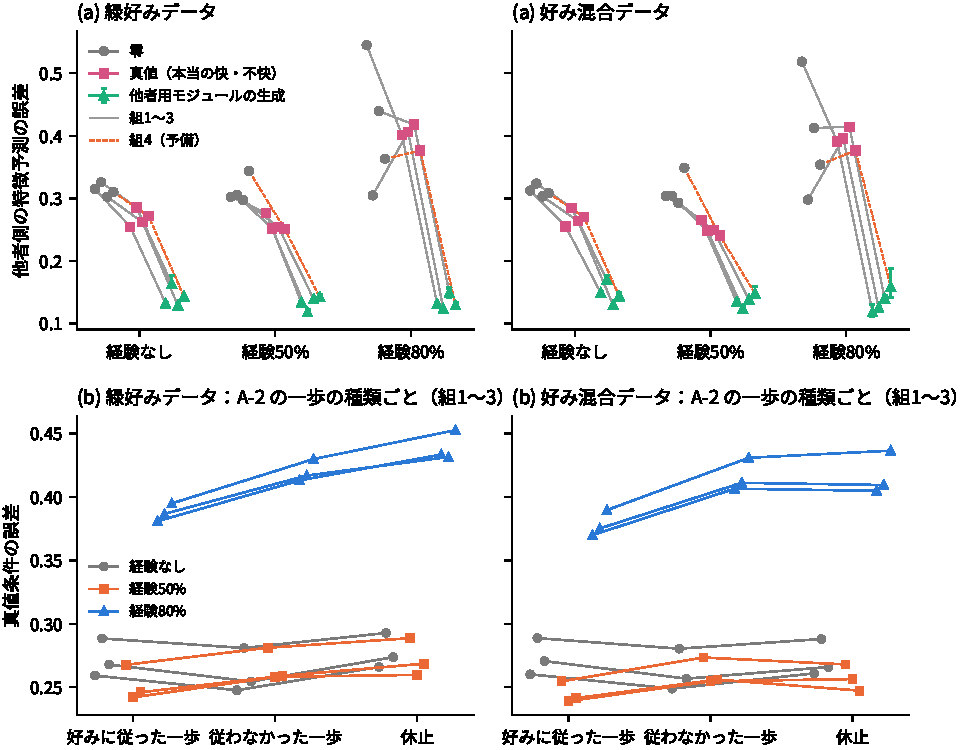
\includegraphics[width=\linewidth]{figs/projection_error}
  % 図4：投影の誤り（実験2の真値条件）。他者側の特徴予測の誤差を，process-2 に零・本当の快・不快（D6）・
  % 他者用モジュールが生成した Q2 を入れた3通りで，経験なし・50%・80% ごとに組別に並べる（組1〜3，組4 があれば足す）。
  % ログに一歩の種類ごとの集計があれば (b) として足す。
  % 元：v13 のログ・まとめの真値条件（T3・D6）の節（Claude Code が README に書く）。
  \caption{他者の本当の快・不快を与えたときの他者側の特徴予測の誤差．(a)(b) 緑好みデータと好み混合データで，process-2 に零，本当の快・不快，他者用モジュールの出力を入れた場合を，経験の量ごとに示す（組1〜3 は灰の実線，組4 は橙の破線）．(c)(d) 本当の快・不快を入れた場合の誤差を，A-2 の一歩の種類（好みに従った一歩，従わなかった一歩，休止）ごとに示す（組1〜3）．}
  \label{fig:projection}
\end{figure}

\begin{table}[t]
  \centering
  \small
  \caption{真値条件における他者側の特徴予測の誤差}
  \label{tab:projection}
  % paper/tables/projection.tex -- generated by analyze/paper/tables_paper.py; sources in paper/tables/README.md
\begin{tabular}{@{}lllllll@{}}
\toprule
 & \multicolumn{3}{l}{緑好みデータ} & \multicolumn{3}{l}{好み混合データ} \\
\cmidrule(lr){2-4}\cmidrule(l){5-7}
条件・組 & 零 & 真値 & 生成 & 零 & 真値 & 生成 \\
\midrule
経験なし・組1 & 0.315 & 0.255 & 0.131〜0.134 & 0.313 & 0.255 & 0.146〜0.151 \\
経験なし・組2 & 0.326 & 0.286 & 0.159〜0.176 & 0.324 & 0.285 & 0.167〜0.177 \\
経験なし・組3 & 0.302 & 0.262 & 0.125〜0.132 & 0.303 & 0.264 & 0.128〜0.131 \\
経験なし・組4 & 0.310 & 0.271 & 0.141〜0.145 & 0.308 & 0.270 & 0.142〜0.149 \\
\midrule
経験50\%・組1 & 0.302 & 0.276 & 0.132〜0.135 & 0.304 & 0.265 & 0.133〜0.138 \\
経験50\%・組2 & 0.305 & 0.252 & 0.116〜0.122 & 0.304 & 0.248 & 0.121〜0.127 \\
経験50\%・組3 & 0.297 & 0.254 & 0.138〜0.142 & 0.293 & 0.249 & 0.138〜0.139 \\
経験50\%・組4 & 0.344 & 0.252 & 0.140〜0.146 & 0.349 & 0.241 & 0.143〜0.159 \\
\midrule
経験80\%・組1 & 0.545 & 0.402 & 0.129〜0.133 & 0.519 & 0.391 & 0.112〜0.130 \\
経験80\%・組2 & 0.305 & 0.406 & 0.121〜0.126 & 0.298 & 0.396 & 0.123〜0.127 \\
経験80\%・組3 & 0.440 & 0.418 & 0.142〜0.157 & 0.413 & 0.414 & 0.134〜0.145 \\
経験80\%・組4 & 0.363 & 0.376 & 0.126〜0.134 & 0.354 & 0.377 & 0.141〜0.188 \\
\midrule[\heavyrulewidth]
\multicolumn{7}{@{}l}{真値条件の誤差を A-2 の一歩の種類で分けたもの（組1〜3 の範囲．括弧は一歩のうちその種類の割合）} \\
\midrule
データ・一歩 & \multicolumn{2}{l}{経験なし} & \multicolumn{2}{l}{経験50\%} & \multicolumn{2}{l}{経験80\%} \\
\midrule
緑好み・好みに従った一歩（0.43） & \multicolumn{2}{l}{0.259〜0.289} & \multicolumn{2}{l}{0.242〜0.268} & \multicolumn{2}{l}{0.381〜0.395} \\
緑好み・従わなかった一歩（0.49） & \multicolumn{2}{l}{0.248〜0.281} & \multicolumn{2}{l}{0.258〜0.281} & \multicolumn{2}{l}{0.413〜0.430} \\
緑好み・休止（0.08） & \multicolumn{2}{l}{0.266〜0.293} & \multicolumn{2}{l}{0.260〜0.289} & \multicolumn{2}{l}{0.432〜0.453} \\
好み混合・好みに従った一歩（0.42） & \multicolumn{2}{l}{0.260〜0.289} & \multicolumn{2}{l}{0.239〜0.255} & \multicolumn{2}{l}{0.370〜0.390} \\
好み混合・従わなかった一歩（0.49） & \multicolumn{2}{l}{0.249〜0.280} & \multicolumn{2}{l}{0.255〜0.273} & \multicolumn{2}{l}{0.407〜0.431} \\
好み混合・休止（0.09） & \multicolumn{2}{l}{0.261〜0.288} & \multicolumn{2}{l}{0.247〜0.268} & \multicolumn{2}{l}{0.405〜0.437} \\
\bottomrule
\end{tabular}

  % 表4：零・真値（D6）・生成した Q2 の誤差を，経験なし・50%・80% ごと，組ごと。
  % 一歩の種類ごとの集計がログにあれば，その行を足す。出典：v13 まとめ §4，v13 ログ §24・§25。
\end{table}

A-2 の本当の快・不快を process-2 に入れたときの他者側の予測の誤差は，経験80\%条件で大きくなり，経験の少ない条件より外れた（図\ref{fig:projection}，表\ref{tab:projection}．経験80\%条件では，段階IIを行った4組のうち2〜3組で，何も与えない場合より悪かった）．
真値条件の他者側の特徴予測の誤差は，段階IIを行った組1〜4 と二つのデータを通して，経験なし条件 0.25〜0.29，経験50\%条件 0.24〜0.28 であったのに対し，経験80\%条件では 0.38〜0.42 であった（表\ref{tab:projection}）．
経験なし条件と経験50\%条件の値はほぼ同じで，大きくなったのは経験80\%条件である．
経験80\%条件で，本当の快・不快を入れた方が何も与えない場合（零を入れた場合）より誤差が大きかったのは，緑好みデータで組2・組4 の2組，好み混合データで組2〜4 の3組であった（追加の比較で測った全6組では，それぞれ3組と4組）．
% 出典：numbers_check.md（Claude Code 第2弾。好み混合の組3：真値 0.4141 対 零 0.4127）。
% 出典：v13 まとめ §4（組1〜3），組4（経験なし 0.272，50% 0.252，80% 0.377，零 0.363）は Claude Code 第1弾の報告と tables/projection.tex。
% 組5・6 は段階IIを行っていないので値がない。
この悪化は予想していなかった結果である．

悪化の大部分は，A-2 がどう動いたかによらない予測の中の位置のずれであると読める（事後の分析による推測）．
経験80\%条件と経験50\%条件の差は，A-2 が好みに従って動いた一歩でも $+0.11$〜$+0.15$ あり，好みに従わなかった一歩や休止の一歩ではそれよりやや大きかった（3組で同じ順．図\ref{fig:projection}(c)(d)）．
% 出典：v13 まとめ §4（「悪化は A-2 が好みに従った一歩でも +0.11〜+0.15 あり，従わなかった一歩・眠りでやや大きい（+0.01〜+0.04，「従った < 従わなかった < 眠り」の順で 3 組そろう）」）。
%   +0.11〜+0.15 が「80%−50%」の差か，+0.01〜+0.04 が何と何の差かは v13 ログ §24・§25 で【要確認】。
また，快・不快を保つ前の時点で，経験80\%条件のモデルは予測の中の A-2 を本当の位置より A-2 の好きな色の方へ寄せて置いていた（$+0.5$〜$+3.7$．経験50\%条件では逆に $-0.7$〜$-1.9$）．
% 出典：v13 まとめ §3.1 の表（止める前の A-2 の置き方。事後の分析）。
経験80\%条件の A-1 は，快が高ければほぼ好きな色の角にいた．
一つの解釈は，その経験から，モデルが他者を自分と同じ強さで快の方へ動く者として見積もり，半分しか好みに従わない A-2 を本当より快の方へ寄せて予測したというものである（自分の行動の仕方の投影）．
寄せる向きは，入れた快・不快の正の向き（A-2 の好きな色）であり，A-1 自身の好きな色ではない．
A-1 自身の好きな色への寄りは，調べた範囲（経験50\%条件のモデルと\ref{app:switch}の好み切替条件）では見られなかった．
% 出典：執筆メモ §5 主張3（v12・v14-C で A-1 自身の好きな色への投影なし），v14 まとめ §3。

ただし，この解釈のほかにも説明が残る．
第一に，段階Iの process-2 には零しか入らないので，本当の快・不快は段階Iのモデルにとって学習で見ていない入力である．
もっとも，同じ入力を入れた経験なし条件と経験50\%条件では誤差は 0.24〜0.29 にとどまり，経験50\%条件では零を入れるよりやや小さかった（零で約 0.30〜0.35）．
したがって，見ていない入力であることだけでは条件の違いを説明できないが，見ていない入力への応じ方が経験の量によって変わった可能性は残る．
第二に，経験80\%条件の学習データの位置の偏りそのものが，他者の位置の予測を角の方へ寄せた可能性がある．
これは自分の行動の仕方の投影と近いが，価値に従って動いた経験ではなく，角に多くいた経験から生じる点で区別される．
評価は全条件で同じデータを用いたので，評価の場面の違いによる説明は当たらない．

\paragraph{他者の行動の仕方を自分にそろえた比較}
そこで，A-2 も 0.8 の割合で好みに従う評価用データで同じ比較を行った（\ref{sec:evaluation}節，図\ref{fig:cross}）．
事前登録した三つの予想は，緑好みデータと好み混合データの両方で，本番の3組すべてと全6組すべてで成り立った．
第一に，経験80\%条件では，A-2 の割合を 0.5 から 0.8 にすると $\Delta$ が小さくなった（本当の快・不快がより役立った）．組をまたいだ変化は，緑好みデータで $-0.096$ [$-0.139$, $-0.054$]，好み混合データで $-0.098$ [$-0.125$, $-0.071$] であった．
第二に，この変化は経験50\%条件より経験80\%条件で大きかった（交互作用 $-0.056$ [$-0.100$, $-0.012$]，$-0.046$ [$-0.072$, $-0.020$]）．
第三に，経験80\%条件と経験なし条件の間の交互作用も同じ向きであった（$-0.071$ [$-0.112$, $-0.030$]，$-0.071$ [$-0.101$, $-0.040$]）．
% 出典：paper_extra_results_log.md（A1・A2・A3，全6組の t の 95% CI，自由度5）。
ただし，A-2 を 0.8 にすると，どの条件でも本当の快・不快はいくらか役立つようになった（A-2 の割合を 0.5 から 0.8 にしたときの $\Delta$ の変化は，組1〜6 と二つのデータを通して，経験なし条件で $-0.016$〜$-0.036$，経験50\%条件で $-0.035$〜$-0.059$，経験80\%条件で $-0.05$〜$-0.16$）．
% 確認：Δ の変化（A-2 0.8 − 0.5）。組ごとの値は paper_extra_results_log.md §A.1・§A.2 の「対比」の表（D_なし・D_50・D_A1）。
また，悪化は消えたのではなく小さくなった．A-2 が 0.8 のとき，経験80\%条件と経験50\%条件の差は，組1・組3 では逆になり（経験80\%条件の方が役立つ），組2・組4・組5 では経験80\%条件の方がまだ悪いが差は小さくなり，組6 では好み混合データで0前後，緑好みデータではまだ悪かった（$+0.032$ [$+0.017$, $+0.047$]）．
また組2 では，A-2 が 0.8 のときにも経験80\%条件で本当の快・不快が零より悪いままであった．
% 出典：numbers_check.md #8・#10（paper_extra_results_log.md §A）。
なお，組1 では A-2 が 0.5 のときにも経験80\%条件で本当の快・不快の方が零より良く，既存の悪化の形は再現されないが，三つの予想の向きは組1 でも成り立った．

この結果は，真値条件の悪化が，自分と他者の行動の仕方の食い違いによって大きく変わることを示す．
学習で見ていない入力であることはどの組み合わせでも同じなので，見ていない入力への不安定さだけでは，この違いを説明できない．
一方，A-2 を 0.8 にすると A-2 も好きな色の角にとどまり，経験80\%条件の A-1 の学習データと位置の分布もそろう．
したがってこの比較では，価値に従って動いた経験の投影と，角に多くいた経験による位置の偏りとは分けられない．
それを分ける対照は\ref{sec:future}節で述べる．
% 出典：v12 まとめ §4 の 3（v12 の T3：零 約0.30，D6 0.25〜0.28）。経験なしの零の値は md にない。

\begin{figure}[t]
  \centering
  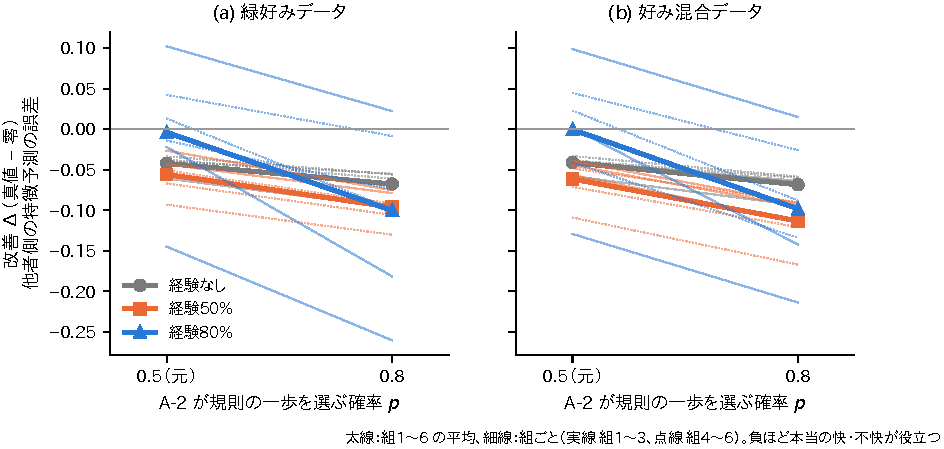
\includegraphics[width=\linewidth]{figs/a_cross_delta}
  % 追加の比較（Claude Code の a_cross_delta.pdf）。横軸は A-2 の規則の割合（0.5／0.8），縦軸は Δ（真値 − 零），
  % 経験なし・50%・80% を線で，組ごとの細い線と全6組の平均。緑好みデータと好み混合データの2パネル。
  % 元：data/result/paper_extra/A_cross/figs/a_cross_delta.pdf（paper/figs/ に写してもらう）
  \caption{他者の行動の仕方を変えたときの，本当の快・不快の役立ち方．縦軸は真値条件の誤差から零を入れた誤差を引いた値 $\Delta$（負なら役立つ）．横軸は A-2 が好きな色へ向かう一歩の割合．(a) 緑好みデータ，(b) 好み混合データ．細い線は各組，太い線は全6組の平均．}
  \label{fig:cross}
\end{figure}

\subsection{実験3：他者用モジュールの学習}\label{sec:res-module}

他者用モジュールは，構成を4通りに変えても他者の好みを書き出さなかった（\ref{app:component}，表\ref{tab:module}）．
事前登録した主の構成（自由出力モジュール，経験50\%条件）では，入れ替え応答 T2 と好み差応答 T5 はともに4組中1組でしか合格の形にならず，不合格であった．
合格の形になった組の値（T2 $+0.03$〜$+0.05$，T5 $+0.04$〜$+0.05$）は，本当の快・不快を入れた値（T2 $+0.60$，T5 $+0.42$）の 1/10 ほどで，組によって向きもそろわなかった．
出力 $Q2$ と本当の快・不快の相関は弱く負に寄り，$Q2$ の分散の 71〜86\% は，本当の快・不快が常に0である範囲 2〜5 が占めていた．
それでも，生成した $Q2$ を入れたときの他者側の特徴予測の誤差（組1〜4，緑好みデータで 0.116〜0.146，好み混合データで 0.121〜0.159）は，本当の快・不快を入れた場合（同じく 0.252〜0.276，0.241〜0.265）よりずっと小さかった．
% 出典：numbers_check.md（Claude Code 第2弾，保存値）。v12 まとめの 0.13〜0.18・0.25〜0.28 は数え方が違う。
モジュールは，予測に役立つ別の情報（範囲 2〜5 を通り道にした他者の位置）を伝えていた．
% 出典：v12 まとめ §3 表2，§4（正式の判定と注意 1〜4）。

この形は，経験80\%条件の段階Iの上で学習しても変わらなかった（探索．T2 は4組中2組，T5 は1組で合格の形．値は $+0.02$〜$+0.05$，$Q2$ と本当の快・不快の相関は4組とも負，分散の 52〜80\% が範囲 2〜5）．
出力を自分が経験した快・不快の形に限った形制限モジュール（T2 は4組中0組），学習データの視界で A-2 を区間ごとに隠した他者遮蔽学習（T2 は3組中0組で，大きく逆向き），出力を1つの符号 $u_t$ に絞った1ビットモジュールでも，好みを書き出す形は出なかった．
1ビットモジュールでは，$u_t$ の符号は正しい候補と偶然より高く一致した（経験50\%条件・経験80\%条件とも，事前登録した判定で3組中3組．経験50\%条件では $u_t$ の平均が好み×配置に沿って入れ替わったが，経験80\%条件では一致の度合いが弱く，BA は 0.51〜0.65）．
しかし，位置をそろえた緑好きと赤好きの A-2 で $u_t$ の違い（T5）はほぼ0で（経験80\%条件で $-0.006$〜$0.000$），好みと方角が食い違うエピソードで $u_t$ が好みに従う割合は経験80\%条件で 0.30〜0.41 と，方角の側に寄った（事前登録した基準で3組中0組が好み）．
1ビットに絞っても，モジュールが書いたのは A-2 の好みではなく，A-2 の進む方角（または位置）であった．
H3 は支持されなかった．
ただし，この結論は調べた4通りの構成，予測の誤差だけによる学習，この課題に限られる．
また，調べたのはモジュールの出力であり，モジュールや共有モジュールの内部状態に好みの情報がないことを示したものではない．
% 出典：v13 まとめ §4（2段目探索），v12 まとめ §3 表2（b 0/4，c 0/3），v14 まとめ §2 (4) 表，v14 ログ §28・§39。
% 1ビットの経験50% の (a)(b) は事前登録していない（v14 ログ §29）ので，本文では経験80% の値を主にした。

\subsection{実験4：仮説の照合}\label{sec:res-inverse}

\begin{figure}[t]
  \centering
  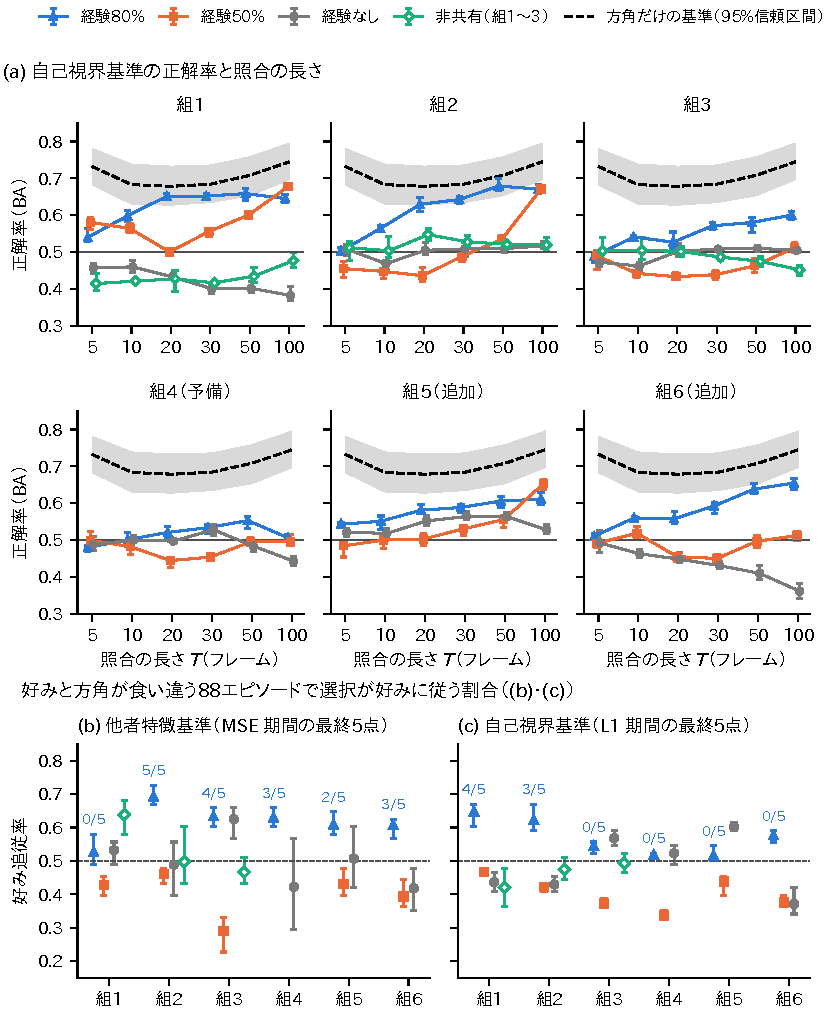
\includegraphics[width=\linewidth]{figs/inverse}
  % 図6：実験4。(a) BA と目標のフレーム数 T（自己視界基準）。経験80%・経験50%・経験なし・非共有条件を組ごとに。
  %   方角だけの基準の BA を同じ軸に描く。0.5 に横線。
  % (b) 食い違う 88 エピソードでの好み追従率（他者特徴基準は MSE 期間の最終5点，自己視界基準は L1 期間）。6組。
  % 元：data/result/v14/summary_figs/fig1_ba_vs_T.png・fig2_follow_pref.png
  \caption{仮説の照合．(a) 自己視界基準での好みの候補の選択の balanced accuracy と，誤差を足し合わせるフレーム数 $T$ の関係（組1〜6．方角だけの基準を並べる）．(b)(c) 好みと方角が食い違うエピソードで選択が好みに従う割合．(b) 他者特徴基準（MSE 期間の最終5点），(c) 自己視界基準（L1 期間の最終5点）．}
  \label{fig:inverse}
\end{figure}

\begin{table}[t]
  \centering
  \small
  \caption{仮説の照合の結果}
  \label{tab:inverse}
  % paper/tables/inverse.tex -- generated by analyze/paper/tables_paper.py; sources in paper/tables/README.md
\setlength{\tabcolsep}{3.5pt}%
\begin{tabular}{@{}lllll@{}}
\toprule
\multicolumn{5}{@{}p{0.9\linewidth}@{}}{(a) 自己視界基準の正解率 BA（$T=50$，L1 期間の最終5点の範囲，括弧は合格の点）} \\
\midrule
組 & 経験80\% & 経験50\% & 経験なし & \\
\midrule
組1 & 0.641〜0.671（5/5） & 0.598〜0.603（5/5） & 0.389〜0.420 & \\
組2 & 0.667〜0.701（5/5） & 0.526〜0.546（0/5） & 0.499〜0.518 & \\
組3 & 0.553〜0.593（4/5） & 0.445〜0.483（0/5） & 0.506〜0.517 & \\
組4 & 0.532〜0.564（2/5） & 0.486〜0.507（0/5） & 0.469〜0.494 & \\
組5 & 0.589〜0.618（0/5） & 0.534〜0.567（0/5） & 0.557〜0.574 & \\
組6 & 0.626〜0.653（5/5） & 0.479〜0.513（0/5） & 0.392〜0.432 & \\
\midrule
方角だけの基準 & \multicolumn{4}{l}{0.708 [0.653, 0.759]（素の一致率 0.707）} \\
 & \multicolumn{4}{l}{規則の一歩が少ない3分の1：0.614 [0.522, 0.704]（117エピソード，素の一致率 0.607）} \\
\midrule[\heavyrulewidth]
\multicolumn{5}{@{}p{0.9\linewidth}@{}}{(b) 経験80\%条件の他者特徴基準の合格の点，好み追従率（他者特徴基準は MSE 期間，自己視界基準は L1 期間の最終5点の範囲，括弧は CI の下限 $>0.5$ の点）} \\
\midrule
組 & 他者特徴基準 & 好み追従率 & 好み追従率 & \\
 & 合格の点 & 他者特徴基準 & 自己視界基準 & \\
\midrule
組1 & 5/5 & 0.489〜0.580（0/5，満たさなかった） & 0.602〜0.670（4/5） & \\
組2 & 5/5 & 0.670〜0.727（5/5，満たした） & 0.591〜0.670（3/5） & \\
組3 & 4/5 & 0.602〜0.659（4/5，満たした） & 0.523〜0.557（0/5） & \\
組4 & 5/5 & 0.602〜0.659（3/5，満たした） & 0.511〜0.523（0/5） & \\
組5 & 5/5 & 0.580〜0.648（2/5，満たさなかった） & 0.500〜0.545（0/5） & \\
組6 & 5/5 & 0.568〜0.625（3/5，満たした） & 0.557〜0.591（0/5） & \\
\midrule[\heavyrulewidth]
\multicolumn{5}{@{}p{0.9\linewidth}@{}}{(c) 経験80\% $-$ 非共有（自己視界基準の BA，$T=50$．組1〜3）：合格の点，ep200 の差 [95\%信頼区間]} \\
\midrule
組1 & \multicolumn{4}{l}{5/5，$+0.255$ [$+0.185$, $+0.324$]} \\
組2 & \multicolumn{4}{l}{5/5，$+0.157$ [$+0.088$, $+0.229$]} \\
組3 & \multicolumn{4}{l}{5/5，$+0.107$ [$+0.037$, $+0.177$]} \\
\bottomrule
\end{tabular}

  % 表5：組1〜6 の経験80%・経験50%・経験なしの BA（自己視界基準，T=50，最終5点の範囲）と合格の点，
  % 他者特徴基準の合格の点，好み追従率の点と書き方（好み／方角），経験80%−非共有（組1〜3），方角だけの基準の BA の行。
  % 出典：v14 まとめ §2 (1)〜(3)，v14_results_log §9。
\end{table}

\paragraph{正解率}
好みの候補を入れ比べて予測誤差の小さい方を選ぶと，経験80\%条件では偶然を上回って A-2 の好みを選べた（図\ref{fig:inverse}(a)，表\ref{tab:inverse}）．
自己視界基準の BA（$T=50$）は，経験80\%条件の本番の3組で $0.553$〜$0.701$ で，3組とも経験なし条件との差が合格の形になった（事前登録した主の判定に合格）．
経験50\%条件では，合格の形になったのは組1だけで（$0.598$〜$0.603$），主の判定は不合格であった．
全6組では，経験80\%条件で4組，経験50\%条件で1組が合格の形になった．
組4・組5 は単独では合格の形にならなかった．
組5では経験なし条件そのものの BA が $0.557$〜$0.574$ と 0.5 を上回り，経験80\%条件との差（$+0.015$ [$-0.040$, $+0.075$]）が出なかった．
また，組1・組6 の差の一部は，経験なし条件の BA が 0.5 を下回ったこと（組1 $0.389$〜$0.420$，組6 $0.392$〜$0.432$）による．
他者側の特徴予測の誤差で選んだ場合（他者特徴基準）も，経験80\%条件の本番の3組で合格の形になった（BA $0.73$〜$0.79$）．
% 出典：v14 まとめ §2 (1) 表，v14 ログ §27 A・B・§43・§44，執筆メモ §5 主張5。

非共有条件では照合は成り立たなかった．
非共有条件の BA は $0.42$〜$0.53$ で，同じ組・同じエピソードの経験80\%条件は3組とも5点すべてで上回った．
非共有条件の選択は，好み×配置に沿って入れ替わらず，一方の候補に偏っていた．
これも構成から予想された確認である．
% 出典：v14 まとめ §2 (3)，v14 ログ §40。

\paragraph{方角で説明できるか}
A-2 の好みは，A-2 がその間に進んだ方角とも結びついている．
A-2 の $t=1$〜50 の変位の向きだけで候補を選ぶと，好みの正解と 0.707 の割合で一致し，BA は 0.708 [0.653, 0.759] であった（方角だけの基準．規則の一歩が少ない3分の1では 0.614 [0.522, 0.704]）．
これは経験80\%条件のモデルの BA（0.53〜0.70）と同じかそれより高い．
したがって，正解率が偶然を上回ったことだけから，モデルが方角以上の手がかりを使ったとは言えない．
なお，方角だけの基準は A-2 の本当の位置を使うのに対し，モデルが使うのは A-1 の視界だけである．
% 出典：v14 ログ §18・§19（0.707），執筆メモ §5 主張5 の注意。BA は第1弾の指示書 §2.1 の 3 で Claude Code が出す。

そこで，好みの正解と方角の正解が食い違う 88 エピソードで，選択が好みに従う割合を調べた（図\ref{fig:inverse}(b)(c)）．
事前登録した条件（他者特徴基準，MSE 期間の最終5点）では，経験80\%条件の本番の3組のうち組2・組3 が好み追従基準を満たし，組1 は満たさなかった．
全6組では，組2・組3・組4・組6 の4組が満たし，組1・組5 は満たさなかった．
自己視界基準（主の判定と同じく L1 期間の最終5点で数えた記述）で同じ割合を見ると，好みに従ったのは6組中2組（組1・組2）であった．
二つの基準のどちらでも好みに従ったのは組2だけである．
経験50\%条件では，どちらの基準でも好みに従う組はなかった（他者特徴基準では，保存された出力のない組4 を除く）．
% 出典：v14 ログ §27 C・§21 B・§21 C，paper/check/follow_pref_late5.json（Claude Code 第1弾）。
% 数え方：v14 まとめ §5 の 3 の「L1 で s0・s1・s5，両方で s1・s5」は，s5 を MSE 期間のチェックポイントで数えたもの。
%   v14 ログ §21 B（MSE 期間の自己の視界の L1 は判定に使わない）に合わせ，L1 期間の最終5点で数え直した（2026-10-26 決定）。

この結果には三つの注意が要る．
第一に，経験なし条件の組3も同じ条件を満たした．
条件を満たすことだけでは経験の効果とは言えない．
第二に，A-2 が規則で動いた一歩が少ない3分の1のエピソードでは，どの組も条件を満たさなかった．
第三に，方角の条件は，経験50\%条件の結果を見た後に作ったものである（経験80\%条件の結果を見る前に登録した）．
方角だけの基準との差（モデルの BA $-$ 基準の BA，同じエピソードで対にしたブートストラップ）を事前登録外の確認として求めた．
主の自己視界基準では，経験80\%条件の差は6組とも負で，組をまたいだ差は $-0.089$ [$-0.140$, $-0.038$] であり，基準を上回った点はどの組にもなかった．
副の他者特徴基準では，経験80\%条件の差は6組とも正で，組をまたいだ差は $+0.049$ [$+0.026$, $+0.072$] と0を含まなかったが，組ごとに信頼区間の下限が0を上回ったのは組4（5点中5点）と組2（5点中2点）だけであった．
同じ他者特徴基準でも，経験50\%条件（$-0.044$ [$-0.087$, $-0.001$]，組4 を除く5組），経験なし条件（$-0.248$ [$-0.357$, $-0.138$]），非共有条件（$-0.260$ [$-0.361$, $-0.159$]，組1〜3）は基準を下回った．
% 出典：paper/check/direction_vs_model.json，paper_round2_log.md §5（Claude Code，測り方 d214f7d，結果 1de3742）。
なお，方角だけの基準は A-2 の本当の位置を使うのに対し，モデルが使うのは A-1 の視界だけである．

以上より，研究者が用意した二つの候補の判別は経験80\%条件で偶然を上回るが（H4 の前半），主の自己視界基準での正解率は方角だけの基準を上回らず，副の他者特徴基準でも組をまたいでわずかに上回るにとどまった．H4 の後半については，一部のモデルで方角に反して好みの側を選ぶ傾向が見られたが，好みに固有の情報による判別は確証されなかった．
方角だけの基準は最終的な変位の向きだけを見るので，位置の履歴や局所的な動きなど，ほかの単純な手がかりを使っている可能性も除けていない．
この結果は，限られた条件での候補の判別として読むべきであり，好みと方角を独立させた課題での確認が要る（\ref{sec:future}節）．
% 出典：v14 まとめ §5 の 1・2，v14 ログ §21・§27 C。

\paragraph{当てて選ぶか，書き出すか}
同じ経験80\%条件の段階Iのモデルで，候補を入れ比べて選ぶ場合（実験4）と，1ビットモジュールに書き出させる場合（実験3）を比べた（図\ref{fig:write-choose}）．
1ビットモジュールを学習した組1〜3 の最終5点で，食い違うエピソードで好みに従う割合は，当てて選ぶと自己視界基準で 0.52〜0.67，他者特徴基準で 0.49〜0.73 と，多くの組で 0.5 を上回った．
書き出させると 0.30〜0.41 で，3組とも 0.5 を下回り，方角の側に寄った．
自分の経験から作られた見込みは，好みの候補ごとに異なる予測を生み，それを観察と照らすと好みをある程度区別できる．
しかし，他者用モジュールに学習させると，モジュールは同じ見込みを使って好みを書くのではなく，予測に役立つ方角や位置を書いた．
% 出典：当てて選ぶ＝Claude Code 第1弾の追加（paper_round1_log.md §7。自己視界基準は L1 期間，他者特徴基準は MSE 期間の最終5点。
%   組1 0.602〜0.670／0.489〜0.580，組2 0.591〜0.670／0.670〜0.727，組3 0.523〜0.557／0.602〜0.659），
%   書き出す＝v14 ログ §39（1ビット 0.30〜0.41，最終5点）。
%   v14 まとめ §2 (4) の 0.55〜0.66・0.57〜0.67 は組1〜3 の L1 期間 ep200 の1点で，数え方が違うので使わない。

\begin{figure}[t]
  \centering
  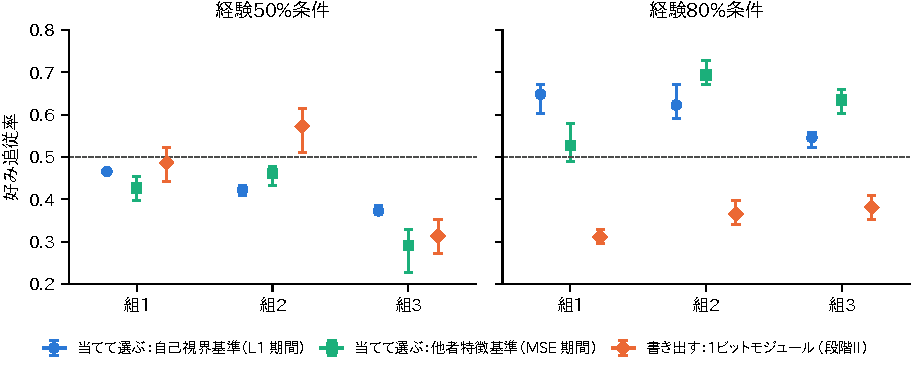
\includegraphics[width=0.8\linewidth]{figs/write_vs_choose}
  % 図5：好みと方角が食い違う 88 エピソードで，選択（または u）が好みに従う割合。
  % 「当てて選ぶ（実験4）」と「書き出す（1ビットモジュール，実験3）」を，経験50%・経験80% で，組ごとに並べる。0.5 に横線。
  % 元：data/result/v14/summary_figs/fig3_write_vs_choose.png
  \caption{同じモデルで，候補を入れ比べて選ぶ場合と，他者用モジュールに書き出させる場合の比較．好みと方角が食い違うエピソードで好みに従う割合を，(a) 経験50\%条件と (b) 経験80\%条件で組ごとに示す．塗りの菱形は事前登録した1ビットモジュールの値，白抜きの菱形は事前登録外の値．破線は 0.5．}
  \label{fig:write-choose}
\end{figure}
